\section{Pruebas}
  Para validar la implementación llevado a cabo, se probará  el sistema operativo con los archivos de prueba create1.c, fork4.c y pingpong.c los cuales son archivos de prueba disponibles en la página web del curso de laboratorio del curso. 
  \subsection{Archivo prueba create1.c}
    \begin{lstlisting}
int main(){
	int fd;
	int e;
        char * buf;
	Create("archivo.nuevo");
	fd = Open("archivo.nuevo");
	Write("prueba", 6, fd) ;
	Close(fd);
//	Exec("../test/rillo");	
	Exec("prueba Exec");

	//char* buf = new int[6];
	fd = Open("archivo.nuevo");
	Read(buf, 6, fd);
	Write(buf, 6, 1);

	Halt();
	return 0;
}      
    \end{lstlisting}
En este caso se prueba los system calls Create, Open, Write, Close, Read y Exec. Como se puede ver en la Ilustración, se ingresa con éxito a los system calls Create, Open y Close. Una vez abierto y cerrado el archivo, envía un mensaje indicando que el archivo se cerró con éxito.
Al ingresar a Exec, muestra que el archivo no se pudo ejecutar dado que no existe. Posteriormente vuelve a abrir el archivo con el SC Open y lee la cantidad de bytes solicitados. En la imagen se muestra que efectivamente esto ocurre.
    \begin{figure}[hbt]
      \begin{center}
        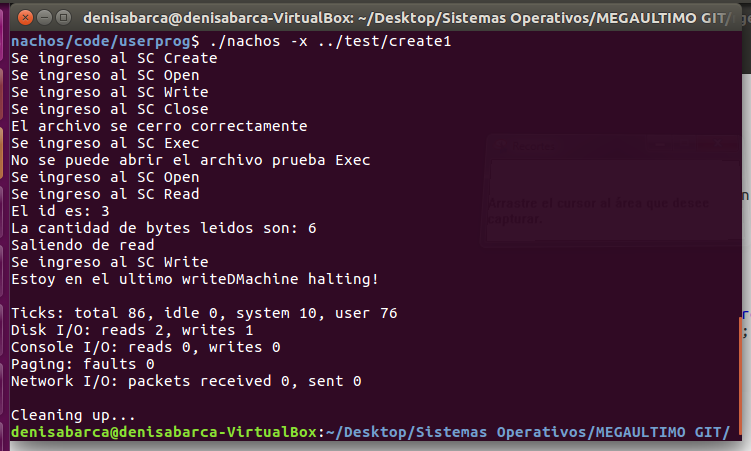
\includegraphics[width=0.5\textwidth]{Prueba_create.PNG}
        \caption{Prueba de create.C}
        \label{fig:create}
      \end{center}
    \end{figure}
\subsection{Archivo prueba: fork4.c}
\begin{lstlisting}
  #include "syscall.h"

void nada(void);
void todo(void);

int semaforoID;

int main(){
	semaforoID = SemCreate(0);
	Fork(nada);
}


void nada(){
	Fork(todo);
	Write("Nada!", 5, 1);
	SemSignal(semaforoID);
}

void todo(){
	Write("Vamos", 5, 1);
	SemWait(semaforoID);
	Write("Final", 5, 1);
}
\end{lstlisting}
En este caso, se prueba el system Call Fork y los system calls asociados a la funcionalidad de los semáforos, es decir; semCreate, semDestroy, semSignal, semCreate. \\
Al inicio, se ingresa con éxito al SC semCreate e inicializa el semáforo en cero. Posteriormente se invoca el System Call Fork. Al crear el Fork la dirección de referencia ejecuta el método void Nada(), en donde al mismo tiempo vuelve a ejecutar el llamado al sistema Fork  ejecutando el método void todo(). \\
En ambos métodos, Vamos y Todo debería ejecutarse los métodos Write mostrando en pantalla los strings ‘Vamos’ y ‘Nada’. Sin embargo, esta prueba presentó el error de que no mostró en pantalla la palabra ‘Nada’ pero sí ‘Vamos’ de los llamados al sistema Write. Lo anterior puede deberse a una falla en la sincronización entre el proceso padre y el proceso hijo.
    \begin{figure}[hbt]
      \begin{center}
        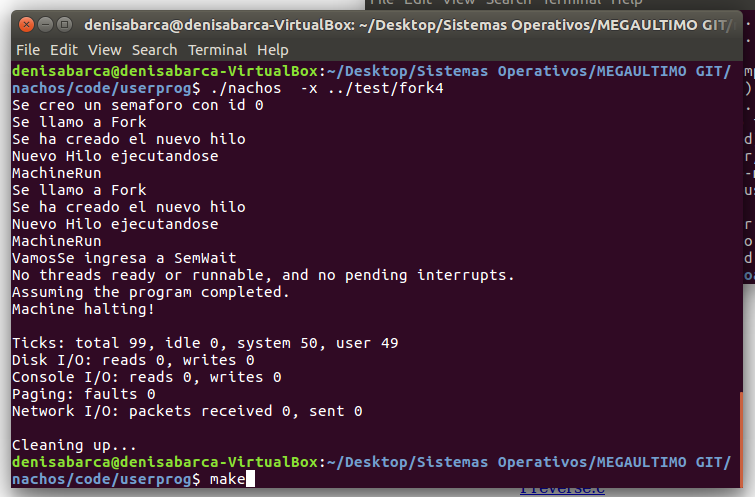
\includegraphics[width=0.5\textwidth]{Prueba_Fork.PNG}
        \caption{Prueba de Fork.C}
        \label{fig:Fork}
      \end{center}
    \end{figure}
    \subsection{Prueba pingPong.c}
    \begin{lstlisting}
#include "syscall.h"

void SimpleThread(int);

int
main( int argc, char * argv[] ) {

    Fork(SimpleThread);
    SimpleThread(1);

    Write("Main  \n", 7, 1);
}

void SimpleThread(int num)
{

    if (num == 1) {
	for (num = 0; num < 5; num++) {
		Write("Hola 1\n", 7, 1);
		Yield();
	}
    }

    else {
	for (num = 0; num < 5; num++) {
		Write("Hola 2\n", 7, 1);
		Yield();
	}
    }
    Write("Fin de\n", 7, 1);
}
\end{lstlisting}
En este caso se analiza la funcionalidad de los métodos Fork y Yield. Consiste en crear un nuevo proceso y posteriormente alternar el hilo que está corriendo empleando el llamado al sistema Yield. \\
Lo primero que ocurre es la creación de un nuevo hilo mediante Fork y posteriormente se llamara al método SimpleThread.\\
Como ahora hay dos procesos e ingresarán a SimpleThread() uno con un valor de argumento igual a 1 y el otro distinto de 1, el llamado al sistema Yield() intercambiará los procesos de manera alternada hasta que se cumple el condicional en el ciclo for. En la Imagen adjunta se muestra que efectivamente esto se logra, ya que Hola 2 y Hola 1 cambian de manera alternada. 
 \begin{figure}[hbt]
      \begin{center}
        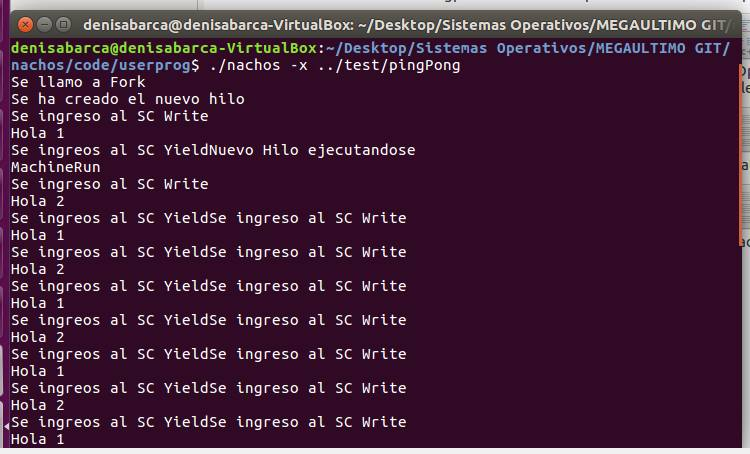
\includegraphics[width=0.5\textwidth]{Prueba_PingPong.PNG}
        \caption{Prueba de Ping Pong.C}
        \label{fig:Fork}
      \end{center}
    \end{figure}
